\section{Experiments}\label{sec:Experiments}
In this section, we evaluate the performance of our proposed method using a representative base-LLM Llama-3.1-8B~\cite{grattafiori2024llama} along with 15 downstream tasks under continue learning regime. We first introduce the datasets, metrics and experimental settings, followed by detailed analyses of the experimental results and landscape visualization~\cite{li2018visualizing,wang2024comprehensive} exploring robustness.

\begin{table}[b]
\footnotesize
\centering
\caption{The statistic of the 15 downstream tasks.}
\label{tab:stats_15tasks}
\begin{tabular}{c|c|c|c}
\toprule
Task Type& Datasets & \# of Train & \# of Test\\
\midrule
SC & yelp & 5000 & 7600 \\
SC & amazon & 5000 & 7600 \\
NLI & MNLI & 3000 & 7600 \\
NLI & CB & 250 & 56 \\
COPA & COPA & 400 & 100 \\
QQP & QQP & 2000 & 7600 \\
NLI & RTE & 2000 & 277 \\
SC & IMDB & 2000 & 7600 \\
SC & SST-2 & 2000 & 872 \\
TC & dbpedia & 14000 & 7600 \\
TC & agnews & 4000 & 7600 \\
SC & yahoo & 10000 & 7600 \\
MultiRC & MultiRC & 2000 & 4848 \\
BoolQA & BoolQA & 2000 & 3270 \\
WiC & WiC & 2000 & 638 \\


\bottomrule
\end{tabular}

\end{table}

\subsection{Datasets}
For the general replay sample set $\mathcal{D}^{\text{(g)}}$, we randomly select 1K samples from the open-source SlimPajama-627B corpus~\cite{cerebras2023slimpajama}, which is a cleaned and deduplicated version of RedPajama~\cite{weber2024redpajama} that reproduces the collection of LLaMA training data.
We release the complete selected samples used throughout this paper to ensure reproducibility. Notably, the selection process is arbitrary rather than deliberately curated (see Appendix for details), which further substantiating the robustness and universality of our method with respect to the replay data.
This replay data potentially reflect the general ability of the base LLM model, which is used to calculate the activation threshold and to compute the threshold-based margin loss.

For the downstream finetuning tasks, we adopt a long-sequence continual learning benchmark comprising as many as 15 diverse datasets~\cite{razdaibiedina2023progressive}, which enables a comprehensive evaluation of model performance in practical scenarios under more demanding and challenging conditions.
The benchmark integrates 5 datasets (yelp, amazon, dbpedia, agnews, yahoo) from the standard CL benchmark~\cite{zhang2015character,qin2021lfpt5}, 4 datasets (MNLI, QQP, RTE, SST-2) from the GLUE benchmark~\cite{wang2018glue}, 5 datasets (CB, COPA, MultiRC, BoolQA, WiC) from the SuperGLUE benchmark~\cite{wang2019superglue}, and the IMDB movie reviews dataset~\cite{maas2011learning}.
In alignment with~\cite{razdaibiedina2023progressive}, we utilize the available validation set for each dataset as the test set since test data is not available.
However, unlike their setting, which randomly selects fixed number of training samples per dataset (i.e., potentially up-sampling or down-sampling), we employ the original full training set for each dataset to better align with real-world scenarios where the data quantity distribution across tasks is inherently imbalanced.
In continual finetuning, we train each task until the training loss converges without validation set.
We proceed to train the next task after the previous one is finish, and the training data for each task was no longer available once used.

Table~\ref{tab:stats_15tasks} presents the dataset statistics for the 15 tasks. Examples mainly including instructions, inputs, and golden answers for each dataset are provided in the Appendix.

\subsection{Metrics}
We evaluate the performance of the final model (i.e., after continual finetuning on 15 tasks) from two dimensions comprising general capabilities and the average accuracy over all downstream tasks.

For general capabilities, We employ MMLU~\cite{hendrycks2020measuring} benchmark, which spans 57 diverse disciplines ranging from STEM, humanities and social sciences, etc., to rigorously measure both factual knowledge and analytical skills across multiple levels of complexity. We use five-shot setting and discriminative evaluation.

For ability to effectively learn the sequential downstream tasks,
we assess the Average Performance (AP)~\cite{chaudhry2018riemannian} of the final model via obtaining task-wise accuracies and then computing their mean. AP reflects the model's overall performance across multiple tasks and its ability to retain knowledge from previously learned.
Notably, we also evaluated the multi-task learning (MTL) regime which finetunes on the combined dataset of all 15 tasks, serving as the theoretical upper bound performance for continual learning.

Finally, we compute the F1 average of the MMLU and AP to reflect the holistic performance of model in maintaining its original general capabilities while effectively learning downstream tasks.
All experimental results are reported as the average of 3 runs.

\begin{figure*}[htbp]
    \centering
    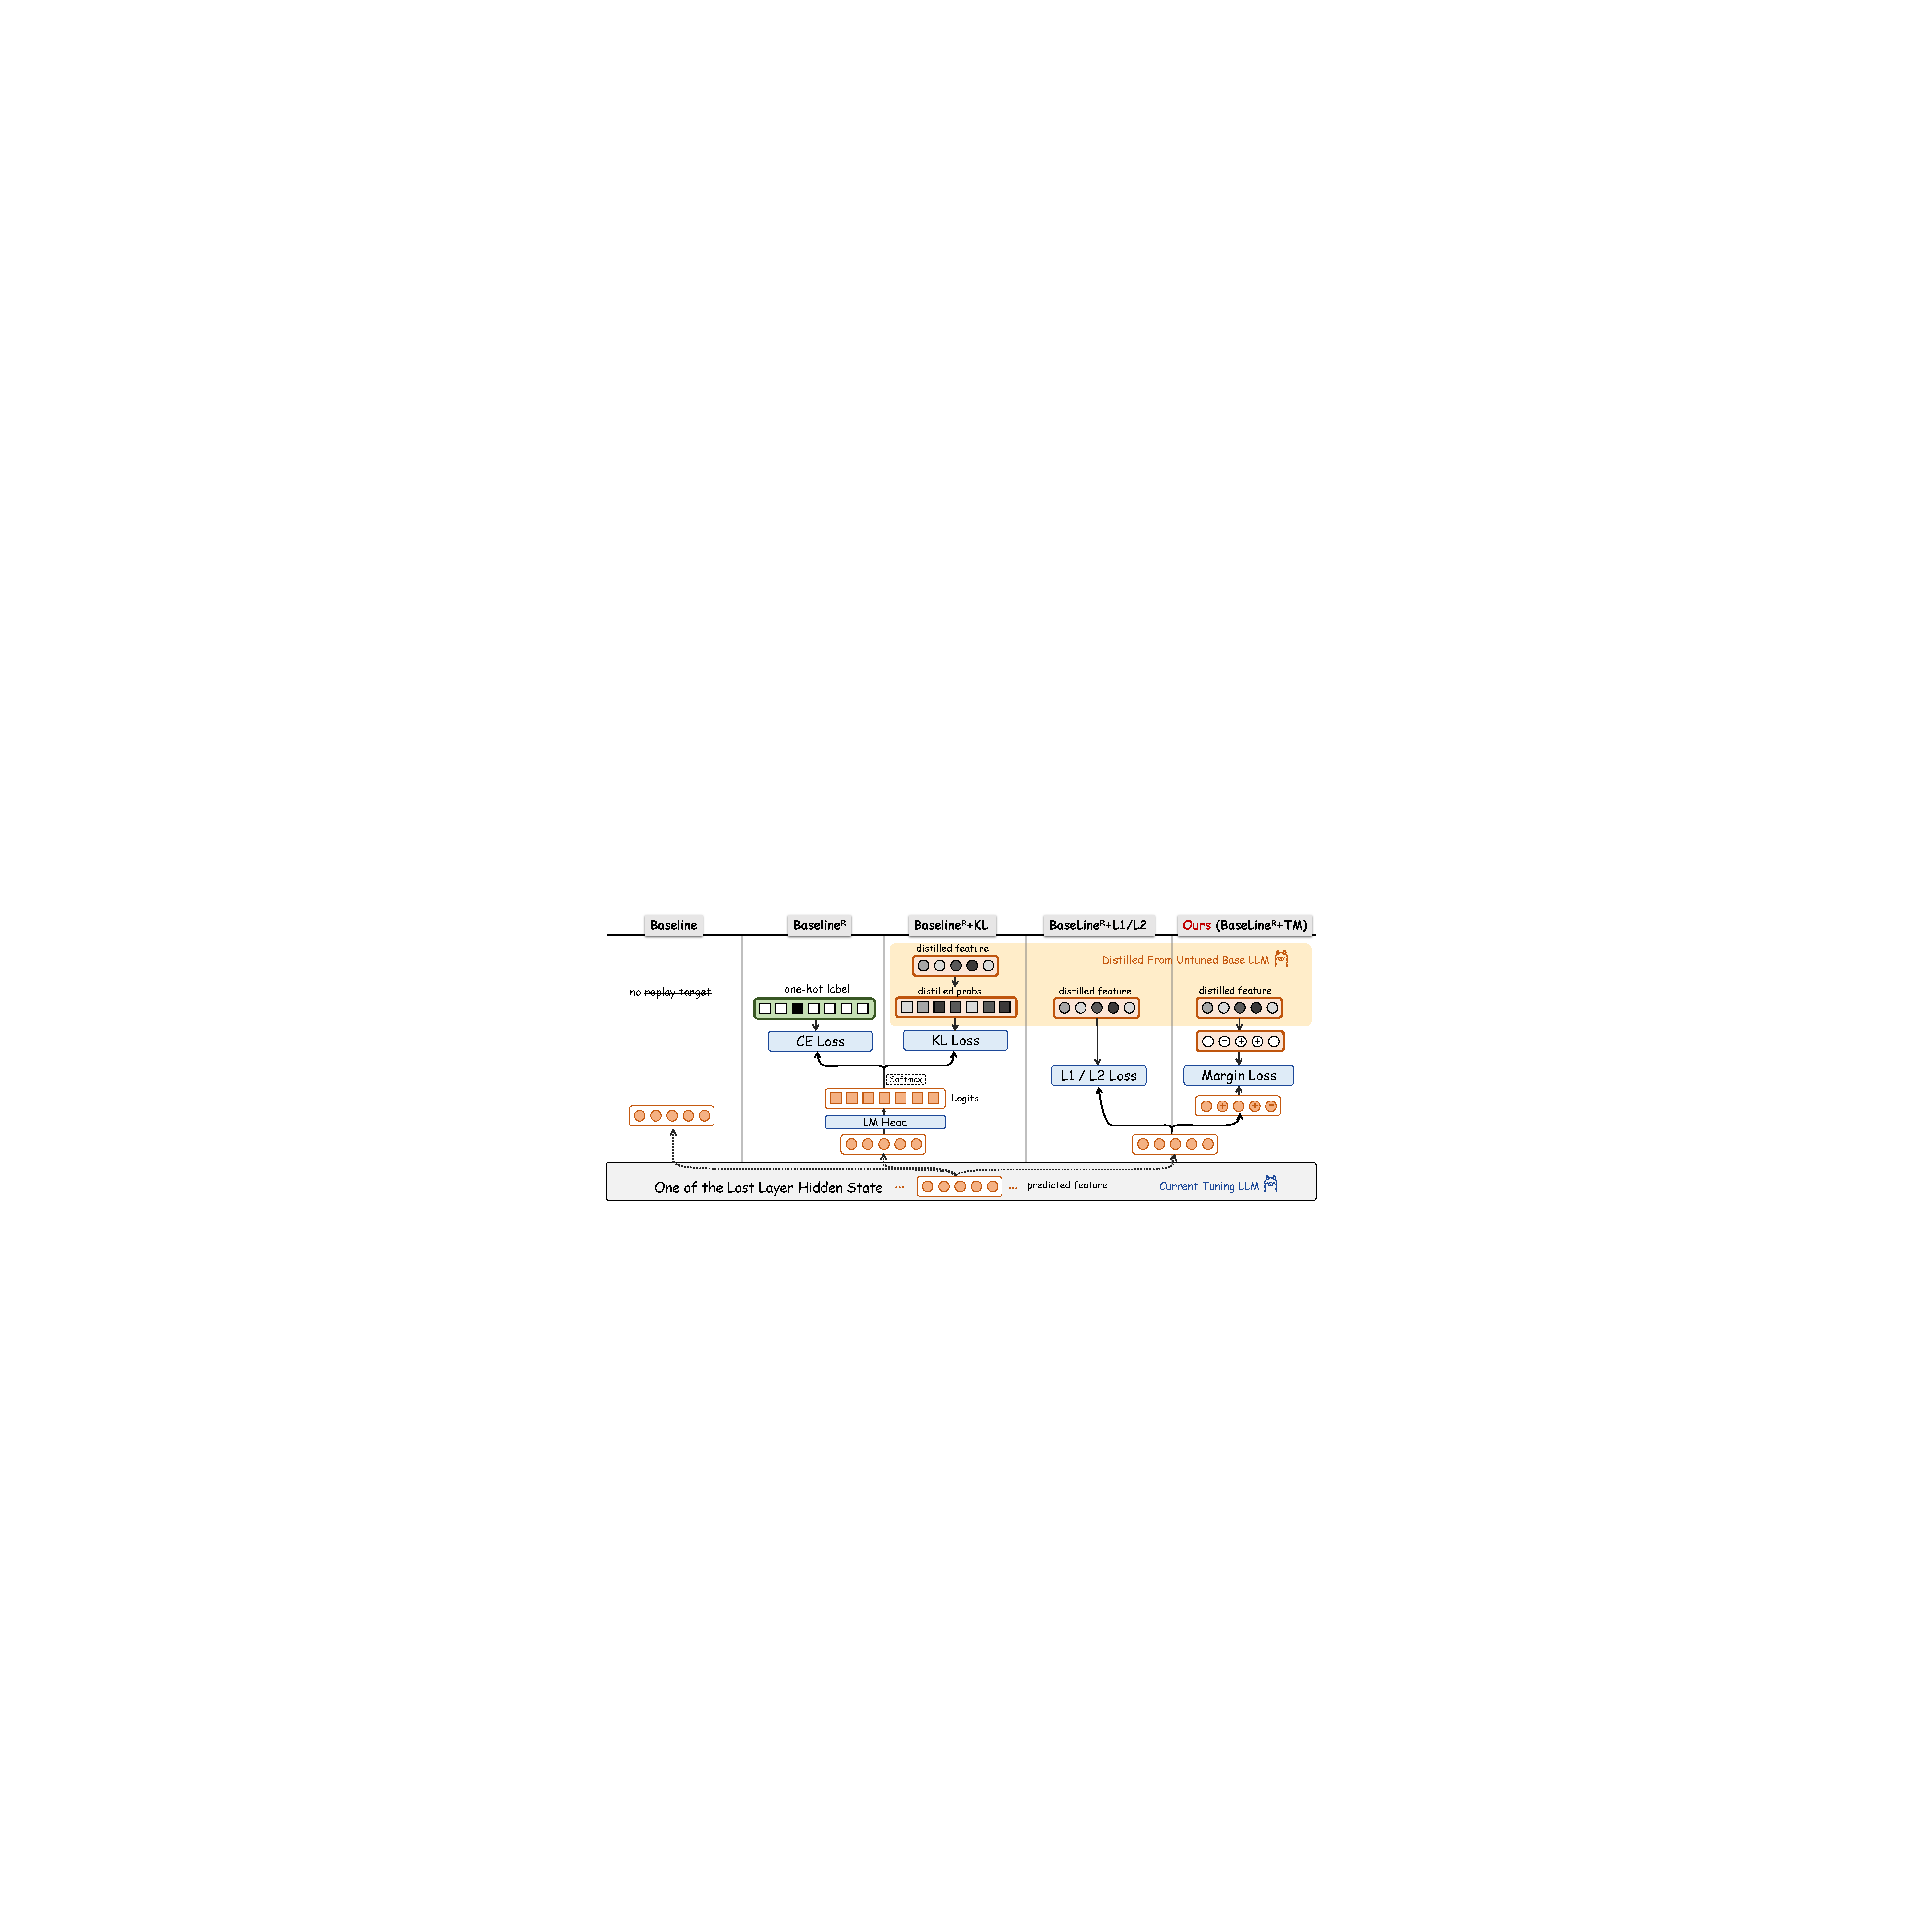
\includegraphics[width=0.8\textwidth]{figtab/compare.pdf}
    \caption{A comparable baseline series of distinct replay-based optimization targets (left to right): native non-replay Baseline, vanilla replay Baseline\textsuperscript{R}, replay with different distillation strategies regarding logits imitation Baseline\textsuperscript{R}+KL and feature imitation Baseline\textsuperscript{R}+L1/L2.
    The rightmost Baseline\textsuperscript{R}+TM is our proposed method, which employs the TM loss.
    }
    \label{fig:compare}
\end{figure*}

\subsection{Comparable Methods}
We meticulously implement all comparable methods from scratch for controlled experiments, including the most basic level and its progressively enhanced counterparts.
As shown in Fig.\ref{fig:compare}, we compare our method (denoted as Baseline\textsuperscript{R}+TM hereafter) with: native non-replay Baseline, vanilla replay Baseline\textsuperscript{R}, replay with different distillation strategies regarding logits imitation Baseline\textsuperscript{R}+KL and feature imitation Baseline\textsuperscript{R}+L1/L2.
These competitors cover the most prevalent and established practices in real-world application.
For fair comparison, all methods are implemented within the same framework using identical replay samples and maintaining consistent configuration throughout the evaluation process. Details are as follows:

\begin{itemize}[leftmargin=*, align=left]
    \item \textbf{Baseline}: continually finetune the LLM on sequential tasks without adding any general replay samples.
    \item \textbf{Baseline\textsuperscript{R}}: continually finetune the LLM on sequential tasks by mixing 1K general replay samples from $\mathcal{D}^{\text{(g)}}$ with each task. These samples are pre-selected before finetuning and remain unchanged throughout the entire finetuning process. Both the replay and downstream task samples are jointly optimized using the standard cross-entropy loss.
    Notably, all the methods discussed subsequently maintain this cross-entropy loss.
    
    \item \textbf{Baseline\textsuperscript{R}+KL}: extend the Baseline\textsuperscript{R} by integrating an additional KL loss.
    Specifically, the pre-distilled general replay sample logits serve as the target for KL loss during finetuning.
    The softmax temperature is set to 2, and the weight of KL loss term is accordingly set to 4 (its square) to compensate for gradient scaling down induced by the temperature~\cite{sun2024logit}.
    In implementation, to avoid the large overhead of pre-storing the high-dimensional $logits$ vectors, we compute the $logits$ in real-time during finetuning based on the previously acquired final layer hidden state $h^\text{(g)}$ and the original $lm\_head$ parameters of LLM.
    
    \item \textbf{Baseline\textsuperscript{R}+L1}: extend the Baseline\textsuperscript{R} by integrating an additional L1 loss computed on the hidden states at the last layer. The previously acquired $h^\text{(g)}$ serves as the target.
    \item \textbf{Baseline\textsuperscript{R}+L2}: resemble Baseline\textsuperscript{R}+L1 but employ L2 loss instead of L1 loss.
\end{itemize}
Our method and other options are explained as follows:
\begin{itemize}[leftmargin=*, align=left]

    \item \textbf{Our method (aka. Baseline\textsuperscript{R}+TM}): extend the Baseline\textsuperscript{R} by integrating our proposed TM loss computed on the hidden states at the last layer as in Eq.\ref{eq:tml}$\sim$Eq.\ref{eq:loss_final}.
    
    \item \textbf{BI Option}: adopt Batch Insertion (Sec.~\ref{sec:BI}) and evaluate its effectiveness across all the replay-based Baseline\textsuperscript{R} series, i.e., Baseline\textsuperscript{R} and Baseline\textsuperscript{R}+KL/L1/L2/TM that typically using general replay samples.

    \item \textbf{Loss Weight}: varied weighting values (denoted as w=[]) of the additional loss term regarding L1/L2/TM are tested. We first empirically set w=1 (omitted as default), w=100 and a dynamic weighting w=d.(Sec.~\ref{sec:DW}) for $\mathcal{L}^{TM}$ to find the optimal performance, and then deliberately evaluate the same optimal weight on L1 and L2 for fair comparison.

    \item \textbf{Upper Bound}: we also include the upper bound performance for comparison, where \textbf{Orig} denotes the original MMLU score of untuned base model as ceiling. \textbf{MTL} denotes a multi-tasks learning result across all 15 downstream tasks, which is trained on the combined task samples with the identical settings (epochs, learning rate, etc.). We calculate their F1 average upper bound as well.
\end{itemize}

\noindent Notably, Baseline\textsuperscript{R}+L1/L2 can be viewed as a stricter version of ours, which pursues precise value fitting (also bringing activation state alignment), but lacks the inherent variation tolerant afforded by our discrete states.

Regarding external competitors, since we strive for a simply yet effective replay-base approach (e.g., prompts-agnostic, task\_ids-agnostic, non-generative), we do not compare with ineligible methods like ProgPrompt~\cite{razdaibiedina2023progressive}, which sequentially integrates previously learned prompts with the current one during both training and testing.
Instead, we compare \textbf{O-LoRA}~\cite{wang2023orthogonal} in our LoRA setting due to its simplicity in only constraining the LoRA's update direction by an additional orthogonal loss term.
We are interested in comparing the downstream tasks performance enhanced as a byproduct by our method with that of the specialized O-LoRA, which is solely dedicated to this purpose.
We reimplement it carefully using the same LoRA hyperparameters.

\begin{table}[hp]
\footnotesize
\centering
\caption{Comparison of different methods on continual full-parameter finetuning (15 epochs per task) in 15 downstream tasks.}
\label{tab:continual_full}
\begin{tabular}{l|c|c|c}
\toprule
\makecell{Methods \\(Full-Parameter)}& \makecell{MMLU Score\\(Final)} & \makecell{15 Tasks AP\\(Final)} & \makecell{F1 Avg} \\
\midrule
\midrule
Baseline &
38.3213& 37.4720& 37.8919\\
\midrule

Baseline\textsuperscript{R} &
50.5332& 39.2741&44.1979\\
\rowcolor{gray!10}\quad w/ BI &
 55.5556&43.9903& 49.1011\\
\midrule

Baseline\textsuperscript{R}+KL &
 51.0492& 42.0231&46.0985\\
\rowcolor{gray!10}\quad w/ BI &
 52.7692 &35.5259&42.4638\\
\midrule

Baseline\textsuperscript{R}+L1 &
 54.9364&66.8605&60.3147\\
\rowcolor{gray!20}\quad w/ BI&
 54.5942& 66.7673&60.0691\\

Baseline\textsuperscript{R}+L2 &
55.0052 & 67.4899& 60.6113\\
\rowcolor{gray!10}\quad w/ BI &
 56.6219& 66.7462&61.2686\\

\midrule
Baseline\textsuperscript{R}+L1 (w=100)&
57.9635&72.4376&64.3973 \\
\rowcolor{gray!20}\quad w/ BI&
59.0299 &71.1125 & 64.5103 \\
Baseline\textsuperscript{R}+L2 (w=100) &
60.7499 &72.6112 &66.1531\\
\rowcolor{gray!20}\quad w/ BI&
57.8947 &73.2265 & 64.6643\\

\midrule
Baseline\textsuperscript{R}+L1 (w=d.)&
53.1132&67.4546&59.4309 \\
\rowcolor{gray!20}\quad w/ BI&
53.2852&64.4925&58.3556 \\
Baseline\textsuperscript{R}+L2 (w=d.) &
55.1772&71.0094&62.1001 \\
\rowcolor{gray!20}\quad w/ BI&
54.7988&68.2590&60.7927 \\

\midrule
\rowcolor{gray!40}
\textcolor{red!80!black}{\textbf{Ours}}& & &\\
Baseline\textsuperscript{R}+TM & 55.3836 &70.3490 & 61.9756 \\
\rowcolor{gray!10}\quad w/ BI & 57.6539& 68.7473&  62.7138\\


Baseline\textsuperscript{R}+TM (w=100) &
60.7155 & 74.0817 & 66.7359 \\
\rowcolor{gray!10}\quad w/ BI &
\textbf{60.9907}&72.4771&  66.2396\\

Baseline\textsuperscript{R}+TM (w=d.) &
60.7843 & \textbf{74.4796} & \textbf{66.9386} \\
\rowcolor{gray!10}\quad w/ BI &
57.2411 & 70.5607 & 63.2068 \\

\midrule
  
Upper Bound &
\makecell{Orig\\ 66.5291} & \makecell{MTL\\ 81.0079} & 73.0580\\

\bottomrule
\end{tabular}

\end{table}


\subsection{Implementation Details}
In all experimental comparison, we assess both full-parameter and LoRA finetuning settings with consistent batch size of 64.
All downstream samples are truncated with a maximum source length of 512 and a maximum target length of 50. Accordingly general replay samples are truncated with a maximum length of summation 562.
In full-parameter setting, we maintain a uniform learning rate of 3e-6 across all methods, employing a warmup strategy coupled with a cosine learning rate schedule.
In LoRA setting, we maintain a uniform learning rate of 1e-4 with warmup strategy across all methods, while seting LoRA hyperparameters to \textit{r}\,=8, \ensuremath{\alpha}=32, LoRA\_dropout=0.1 and only tuning the parameters limited to $q\_proj$ and $k\_proj$.
We aim to finetune each task with sufficient steps to ensure loss convergence. Based on preliminary experiments, we ultimately selected 15 epochs per task for the full-parameter setting (due to the smaller learning rate) and 8 epochs for the LoRA.

Notably, the replay samples used in all experiments are identical (the pre-selected set of 1K samples mentioned in Baseline\textsuperscript{R}), which guarantees that the observed effects are attributable to the methodological variations rather than differences in the replay data.
All experiments are conducted using Transformers~\cite{wolf2020transformers} library with DeepSpeed ZeRO-2~\cite{rajbhandari2020zero} and AdamW optimizer~\cite{loshchilov2017decoupled}, running on up to 8 H800-80GB GPUs.

For the BI option experiments, we set $\rho^{\text{BI}}$=$4/64$, which indicates that 4 general replay samples are inserted into each batch of 64 data points. Specifically, these 4 general replay samples are selected randomly and non-repetitively from the aforementioned 1K samples. Once all samples have been selected, the process is reset to ensure continuously sampling.

\subsection{Results}

\subsubsection{Continual Full-Parameter Finetune}
Table~\ref{tab:continual_full} shows the performance of each method in continual full finetuning 15 downstream tasks.
We find that simply mixing general replay samples (Baseline\textsuperscript{R}) significantly outperforms the Baseline without any replay, achieving a notable improvement of 12\% on MMLU. It justify the widespread adoption of this vanilla replay way in practice.

After additional distillation technique, Baseline\textsuperscript{R}+KL yields further improvements by capturing more information, specifically the distribution of labels.
However, under the similar distillation cost, feature-based methods (Baseline\textsuperscript{R}+L1/L2/TM) perform remarkable better,
empirically suggesting that feature information is more efficient than label information by encoding richer representations of model knowledge in feature layer.
Our rationale is that softmax-normalized labels tend to be dominated by extreme values, whereas features preserve finer-grained details.
Among them, Baseline\textsuperscript{R}+TM further alleviate the overly rigid inherence of L1/L2 loss by appropriately constraining optimization from an activation state perspective, achieving the highest performance.

Moreover, the results of all Baseline\textsuperscript{R} series validate the hypothesis that using only general replay samples can simultaneously maintain general capabilities and enhance overall performance of downstream task. As shown in the table, both MMLU and AP improve.
This provides an alternative to the traditional practice of laboriously collecting downstream task replay samples during continual finetuning, sparking a promising research direction.

\begin{table}[t]
\footnotesize
\centering
\caption{Comparison of different methods on continual LoRA finetuning (8 epochs per task) in 15 downstream tasks (w=d. denotes weight dynamic).}
\label{tab:continual_lora}
\begin{tabular}{l|c|c|c}
\toprule
\makecell{Methods \\(LoRA)}& \makecell{MMLU Score\\(Final)} & \makecell{15 Tasks AP\\(Final)} & \makecell{F1 Avg} \\

\midrule
\midrule
Baseline &
55.7620 & 73.3944 & 63.3746\\
\midrule
Baseline\textsuperscript{R} &
58.6515& \textbf{75.5310}& 66.0296\\

\rowcolor{gray!10}\quad w/ BI &
56.5187& 73.3986& 63.8621\\
\midrule

Baseline\textsuperscript{R}+KL &
61.0251& 74.8367& 67.2289\\

\rowcolor{gray!10}\quad w/ BI &
61.5755& 72.9626& 66.7872\\

\midrule
Baseline\textsuperscript{R}+L1 &
61.5411& 73.4170& 66.9565\\

\rowcolor{gray!10}\quad w/ BI &
65.1875& 73.1178& 68.9253\\

Baseline\textsuperscript{R}+L2 &
61.6787& 74.9397& 67.6656\\

\rowcolor{gray!10}\quad w/ BI &
64.4651& 74.1000& 68.9476\\


\midrule
\rowcolor{gray!40}
\textcolor{red!80!black}{\textbf{Ours}} & & &\\
Baseline\textsuperscript{R}+TM &
65.3251 & \textbf{75.0639}& \textbf{69.8567} \\
\rowcolor{gray!10}\quad w/ BI &
64.6371 & 72.7650 & 68.4606\\

Baseline\textsuperscript{R}+TM (w=100) &
65.9443& 63.9167& 64.9147 \\
\rowcolor{gray!10}\quad w/ BI &
65.5659& 68.7755& 67.1323\\


Baseline\textsuperscript{R}+TM (w=d.) &
\textbf{66.2539}& 64.4417&65.3352 \\
\rowcolor{gray!10}\quad w/ BI &
65.4627& 67.7580& 66.5906\\


\midrule
O-LoRA~\cite{wang2023orthogonal} &
55.8996 & 73.6823 & 63.5707\\

\midrule
Upper Bound &
\makecell{Orig\\ 66.5291} & \makecell{MTL\\ 80.3474} & 72.7882\\

\bottomrule
\end{tabular}

\end{table}

\subsubsection{Continual LoRA Finetune}
Table~\ref{tab:continual_lora} shows the performance of each method in continual LoRA finetuning 15 downstream tasks.
Compared to full-parameter setting, LoRA alone exhibits notable superiority, which tunes only 0.042\% of the parameters (i.e., $q\_proj$ and $k\_proj$), This minimal parameter tuning likely contributes to its strong anti-forgetting ability, but it still enables adequate learning of new tasks.
For instance, when equipped with LoRA, both the Baseline and vanilla replay Baseline\textsuperscript{R} nearly match the best F1 Avg observed in full-parameter, and Baseline\textsuperscript{R} also show surprisingly strong AP of downstream tasks.
Still, similar trends hold for LoRA, with the Baseline\textsuperscript{R} series showing progressive improvements, where our method ultimately achieves the best F1 Avg.
We also find that several methods here have achieved MMLU scores nearly matching the upper bound evaluated from original base model, showing negligible loss of general capabilities.

O-LoRA, as a simple and comparable approach dedicated to AP of downstream tasks, achieves decent AP performance but exhibits obvious forgetting of general capabilities. Furthermore, the original O-LoRA paper claims its superiority over the method with replaying downstream task samples, but we still attain a higher AP. This demonstrates the multifaceted advantages of our GeRe framework over tradition.

By the way, the MTL performance under both settings shows that LoRA still slightly underperforms full-parameter when jointly learning multiple new tasks, aligning with study\cite{biderman2024lora} and suggesting that full-parameter remains preferable in normal situation with available computational resources.

\subsubsection{Ablation Study of BI and Loss Weight}
Each method with BI option under full-parameter and LoRA settings is additional list in Table.\ref{tab:continual_full}$\sim$\ref{tab:continual_lora}.
The effectiveness of BI varies across methods and settings, without showing consistent enhancement. For instance, BI improves the Baseline in full-parameters and Baseline\textsuperscript{R}+L1/L2 in LoRA, but its effect appears negligible in most distillation methods that already capture more information.
We attribute this to the small scale of our finetuning datasets in the experiments, where mixing 1K general replay samples suffices for many downstream tasks. In extremely small datasets like CB, BI’s proportional insertion may even reduce the final replay samples below the standard 1K.

However, BI remain necessary in potential scenarios especially finetuning large-scale downstream task datasets that may far exceeds the 1K replay samples. In such cases, data balancing is crucial since simply mixing them at their original scale leads to insufficient replay. 
As shown in the results, while BI does not significantly improve performance, it also does not degrade it especially with our method, indicating that Baseline\textsuperscript{R}+TM with BI can be directly used in most circumstances.
In conclusion, the adoption of BI should be determined by practical considerations and an optimal replay insertion ratio, which warrants further investigation

Regarding different loss weight, the results also vary.
In full-parameter setting, our method with dynamic weighting $\mathcal{L}^{TM}$, i.e., Baseline\textsuperscript{R}+TM (w=d.) performs best, even in a fair comparison where L1 and L2 are purposefully evaluated with the same weighting strategy.
In contrast, a simply setting of fixed weight of 1 yields better performance under LoRA, as larger or dynamic weight tend to degrade AP. So We only list results (w=1) of L1 and L2 as well. This indicates that different settings should better have their individual weight strategies, and we have already explore two best practice. Unified settings remain for future research. In the following comparison, we intentionally use results of w=100 for full-parameter setting and w=1 for LoRA in order to simultaneously consider the maximum achievable performance of the L1/L2 competitors.

Furthermore, conventional belief suggests that strengthening the weight of optimization direction toward anti-forgetting will enhance stability at the cost of plasticity, thereby impairing learning of new task. However, results with higher weight (from w=1 to w=100) show that not only MMLU dose but also downstream task's AP continues to improve. This may stem from the adoption of general replay samples rather than task-specific replay samples, which mitigates the Stability-Plasticity Dilemma \cite{dohare2024loss} typically occurs when excessively replaying samples from downstream tasks in tradition.

\begin{figure*}[htbp]
    \centering
    \includegraphics[width=\textwidth]{figtab/trend.pdf}
    \caption{Performance trend during continual learning 15 tasks of different methods. Y-axis of each figure indicates the specific task that has just been learned. Two rows depict full-parameter and LoRA settings, respectively. Three columns are metrics: current MMLU score, average performance over tasks learned so far, F1 average.}
    \label{fig:over_tasks}
    \vspace{-10pt}
\end{figure*}


\begin{figure}[htbp]
    \centering
    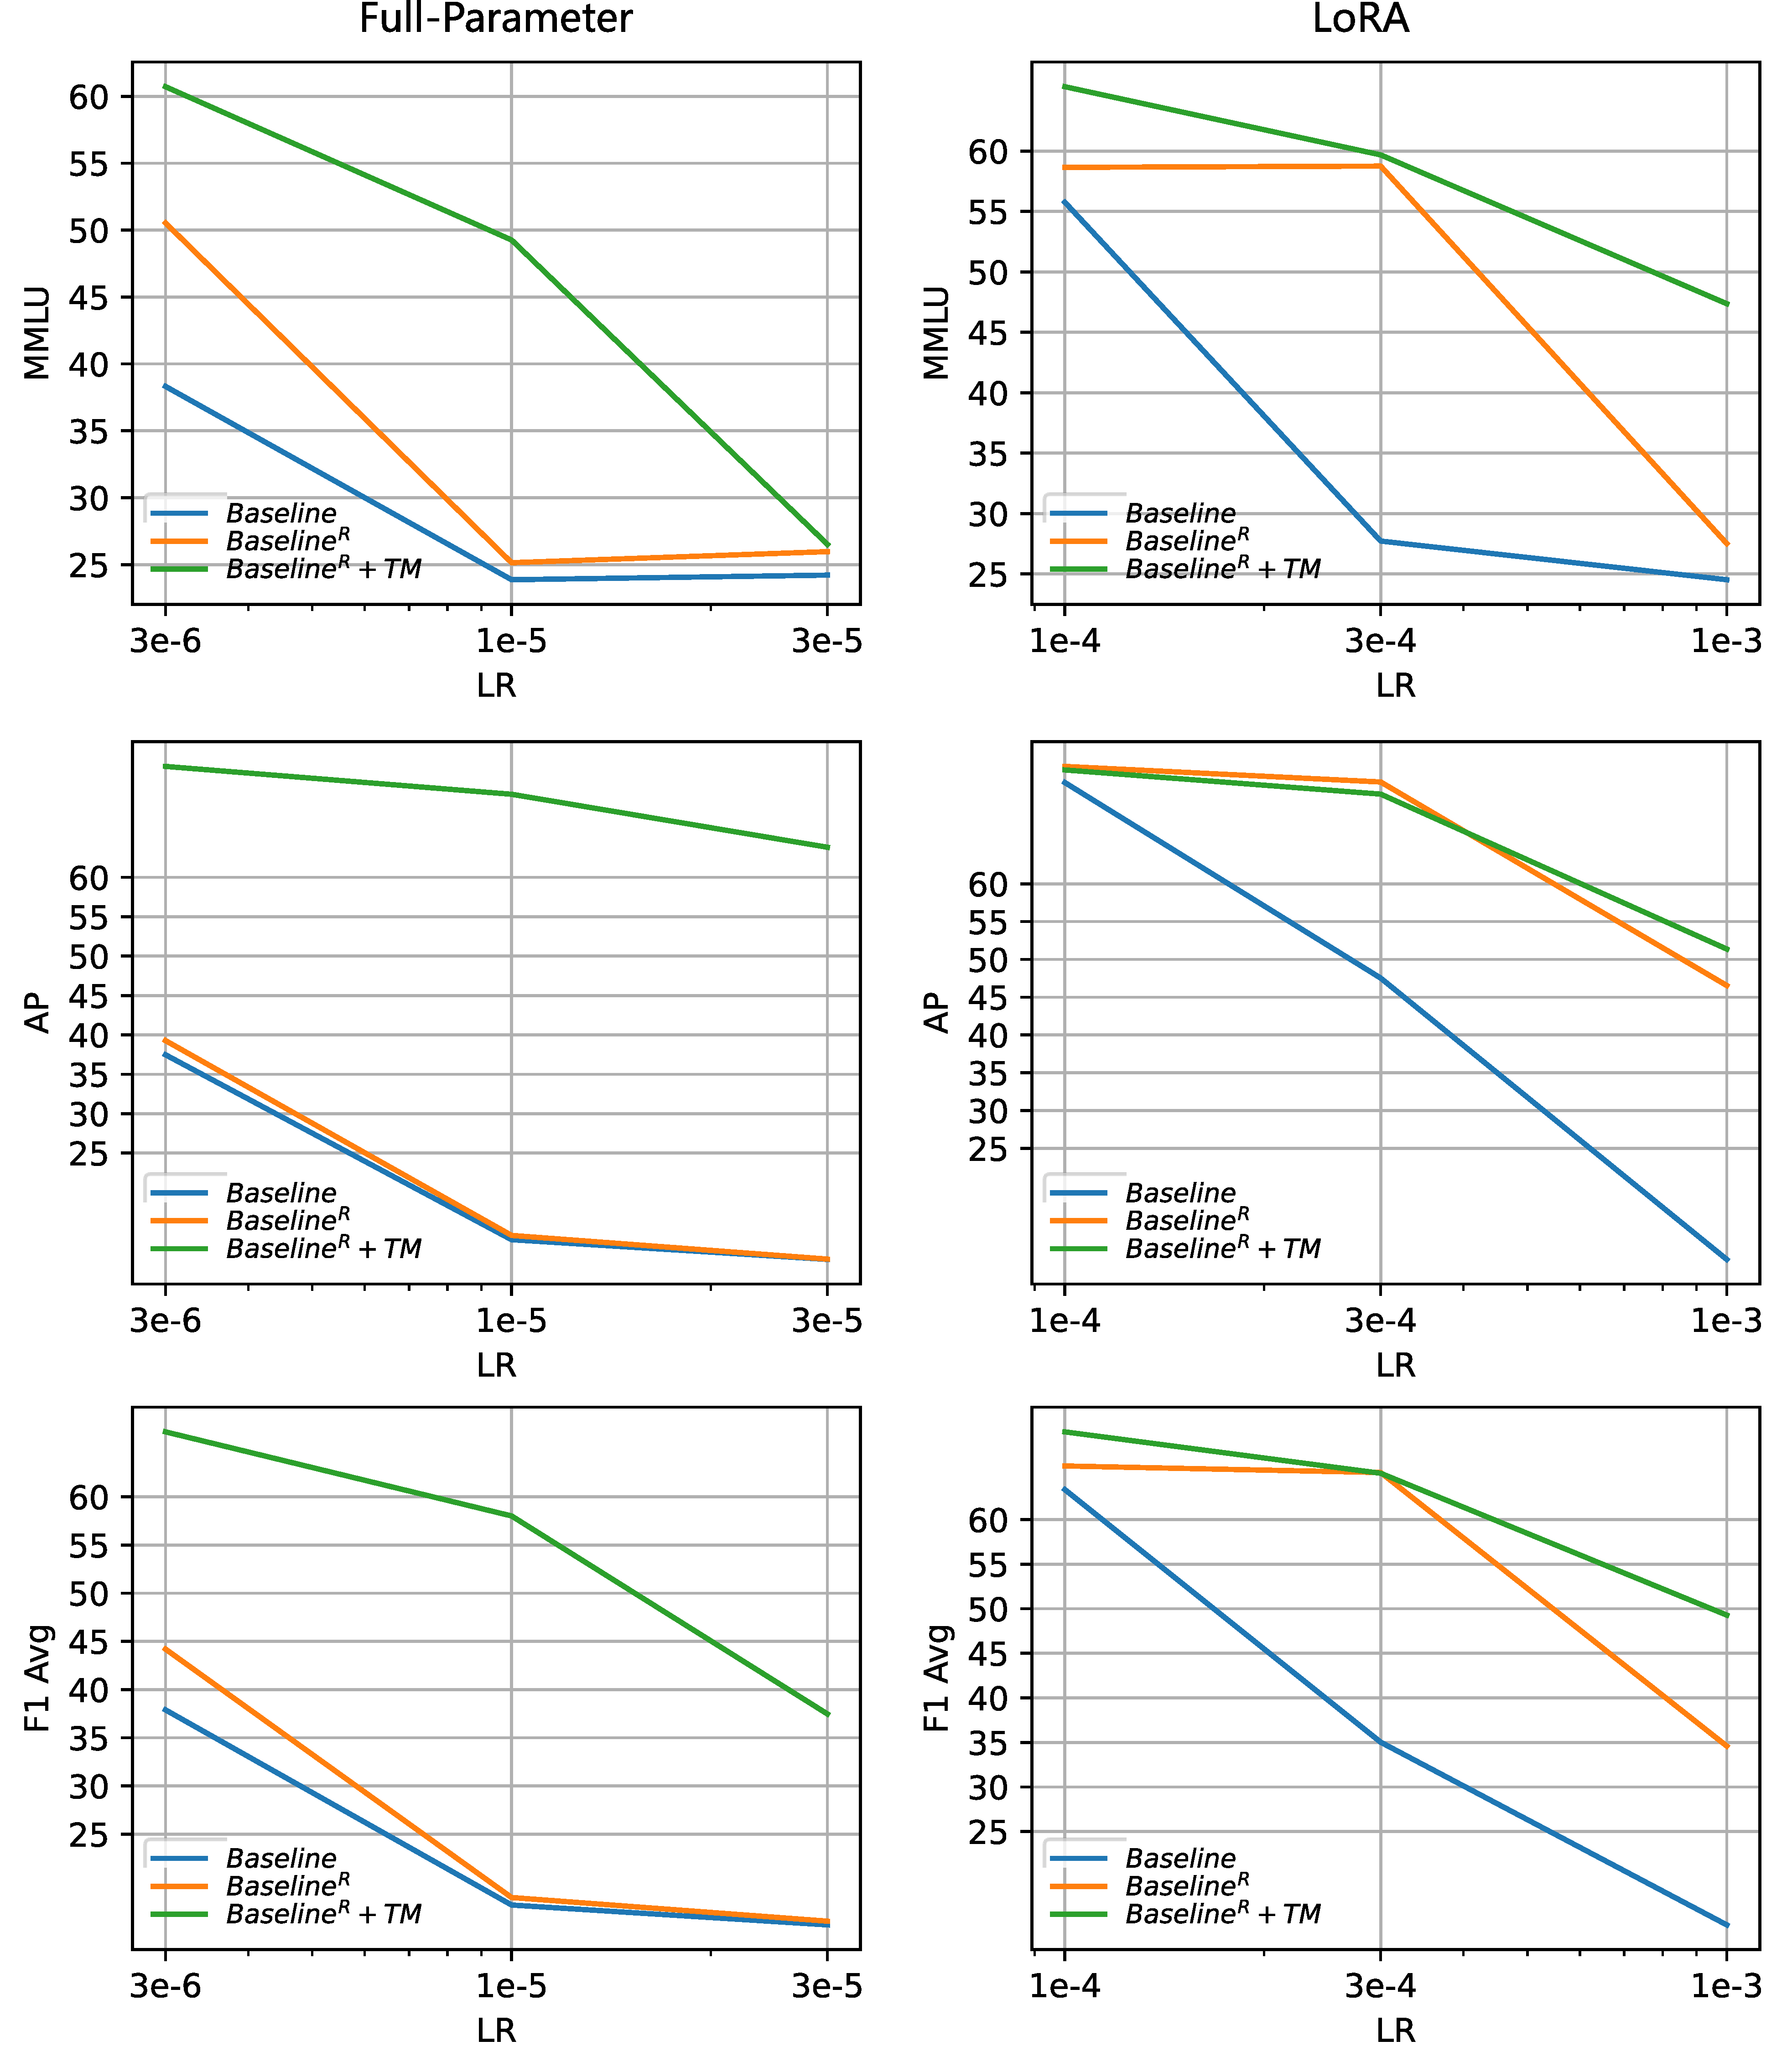
\includegraphics[width=0.9\columnwidth, height=8.5cm]{figtab/lr.pdf}
    \vspace{-8pt}
    \caption{MMLU, AP and F1 Avg performance of three major representative methods across different learning rate is compared under full-parameter and LoRA settings, with the LR axis displayed on a logarithmic scale.}
    \label{fig:lr_robustness}
    \vspace{-10pt}
\end{figure}


\begin{figure*}[ht]
    \centering
    \includegraphics[width=1\textwidth]{figtab/landscape_full.pdf}
    \caption{Landscapes of (a) replay samples loss, and (b) MMLU score under \textbf{full-parameter setting}.
    Origin point (0,0) is base untuned model.
    Y-axis is weight update direction of Baseline (0,1), representing the learning dedicated to downstream tasks.
    X-axis is weight update direction of target method for comparison (1,0).
    % replay-based Baseline\textsuperscript{R} series
    The upper-right area of interest simulates the target model guided by the learning direction of downstream tasks (yellow arrow), where the flatness (see zoomed-in view) can imply the optimizing robustness against latent forgetting even under potential overtraining in practice.
    }
    \label{fig:landscape_full}
\end{figure*}

\begin{figure*}[ht]
    \centering
    \includegraphics[width=1\textwidth]{figtab/landscape_lora.pdf}
    \caption{Landscapes of (a) replay samples loss, and (b) MMLU score under \textbf{LoRA setting}.
    Origin point (0,0) is base untuned model.
    Y-axis is weight update direction of Baseline (0,1), representing the learning dedicated to downstream tasks.
    X-axis is weight update direction of target method for comparison (1,0).
    The upper-right area of interest simulates the target model guided by the learning direction of downstream tasks (yellow arrow), where the flatness (see zoomed-in view) can imply the optimizing robustness against latent forgetting even under potential overtraining in practice.
    }
    \label{fig:landscape_lora}
\end{figure*}

\subsubsection{Performance Trend Over Tasks}
Fig.\ref{fig:over_tasks} shows the dynamic changes of the three metrics assessed in Table \ref{tab:continual_full}$\sim$\ref{tab:continual_lora} as the model sequentially learns 15 downstream tasks under full-parameter and LoRA settings.
Evidently, our method consistently achieves the highest score on MMLU at nearly every task step under both settings. Moreover, it remains in the top tier performance of AP across the downstream tasks learned so far, achieving the best final F1 Avg.

Notably, during the full-parameter learning, a significant decline in AP occurs after the model learned the COPA task.
A Deeper investigation of the task-wise results (see Appendix) reveals that it is mainly caused by performance drops in the MNLI and CB tasks.
We attribute this to the unique instruction format of COPA without providing options (see Appendix), which temporarily disrupts the model's instruction-following ability after learning COPA.
So, tasks with the most similar instructions like MNLI and CB experience performance degradation.
Fortunately, as the model continues to learn subsequent tasks with regular instructions, the performance of these two tasks recovers. We interpret this as a case of spurious forgetting~\cite{zheng2025spurious}, where the model does not lose the core knowledge of these tasks but undergoes temporary confusion in instruction following, which can be readily restored in later learning phases.

\subsubsection{Robustness to Learning Rate}
In continual finetuning, it is well-established that while larger learning rates (LR) facilitate more thorough learning of downstream tasks, they also intensify the forgetting of previously acquired knowledge.
This effect becomes particularly pronounced when dealing with LLMs featuring massive training parameters, which aligns with our observations in preliminary experiments.
Thus, practitioners need to carefully adjust the LR from relatively small values to balance new task acquisition with knowledge retention. 

However, empirical evaluating against both the native Baseline and vanilla replay Baseline\textsuperscript{R} show that our method maintains relatively strong general capabilities (MMLU scores) even with substantially increased LRs.
As shown in Fig.\ref{fig:lr_robustness}, our method gains more stable performance despite a 3× LR increase under full-parameter and a 10× increase under LoRA.
In contrast, the compared methods approach a MMLU score of nearly 25\% ,equivalent to random guessing among 4 options, highlighting their vulnerable dependence on tuning LR.
Our methods demonstrates superior adaptability in practice scenarios.
Beyond MMLU, similar conclusions regarding AP and the resulting F1 Avg can be drawn from the subsequent subfigures.

\subsubsection{Robustness in Optimization Landscape}
To better understand the underlying optimization mechanisms of different methods and their robustness against forgetting, we visualize the landscapes with two contour values under full-parameter (Fig.\ref{fig:landscape_full}) and LoRA settings (Fig.\ref{fig:landscape_lora})

Our idea is that in replay-based learning, to ensure thorough learning for downstream tasks, excessive training can easily occur, which will compromise the general capabilities.
We consider that a better method should reconcile the optimization directions of both downstream tasks and replay samples. Such a method would maintain latent robustness even when subjected to excessive downstream task training that typically induces forgetting.
According to task vector arithmetic~\cite{ilharco2023editing}, we can directly perform linear combinations of model weight for a specific method to simulate and observe their robustness to optimization dynamics under extreme conditions of excessive training. 
Therefore, the landscape is designed as a 2D weight space spanned by two specific model weight update directions, where y-axis is the update direction of the Baseline and x-axis is one of the interested methods for comparison.
Specifically, the upward direction (yellow arrow) indicates the optimization toward native continual finetuning without any replay, highlighting exclusive learning of downstream tasks.
The rightward direction indicates the optimization toward a target model trained from a specific method among the replay-based series.
Based on this coordinate, the upper-right region (white rectangle) is the area of interest that can reveal the robustness against forgetting undergoing potential overtraining, as it simulates the weight update direction imposed on the target model toward overly optimizing downstream tasks.

As for contour values, we select two metrics: a) the CE loss of replay samples, as it is universally adopted and optimized across all methods, and b) the direct MMLU score for straightforward observation. These values measure the retention of general capabilities implicitly and explicitly, respectively. The flatness (i.e., the rate of performance degradation) of the area of interest indicates how robustly each method preserves their general capabilities while learning downstream task.

The landscapes are implemented with positioning the untuned base LLM model at coordinate (0,0), the native Baseline finetuned model at coordinate (1,0), and a specific replay-based finetuned model for comparison at coordinate (0,1).
Weight parameters of each model are flattened into a vector, and the two basis vectors of this coordinate system are derived by subtracting the corresponding model weight vectors
(e.g., $\vec{\mathbf{y}}{=}\mathbf{w}_{\text{[target]}}{-}\mathbf{w}_{\text{base}}, \vec{\mathbf{x}}{=}\mathbf{w}_{\text{baseline}}{-}\mathbf{w}_{\text{base}}$).
We use these two basis vectors to generate a grid of points, where each point represents a model derived from a linear combination of these basis vectors
(e.g., (0.6,0.4) denotes model of weight $\mathbf{w}{=}0.6\vec{\mathbf{x}}{+}0.4\vec{\mathbf{y}}$).
For every model associated with the points, we compute the loss of replay samples and the MMLU score, creating the contour plot as landscape, respectively.

For instance, Fig.\ref{fig:landscape_full}(a) shows the replay sample loss under full-parameter setting.
We observe that the Baseline\textsuperscript{R} exhibits a notably steepness in the area of interest, implying that this optimization encounters significant conflicts when following the direction of learning downstream tasks while attempting to replay to retain general capabilities. This potentially accounts for its poor performance in Tab.\ref{tab:continual_full}.
The same issue persists in Baseline\textsuperscript{R}+KL, though it is relatively less severe, but still remarkable.
In comparison, the feature-based replay methods show significantly flatter behavior in the area of interest, and among them our Baseline\textsuperscript{R}+TM performs the flattest upon closer look at the contour values in the zoomed-in view. This mean our method show better robustness to the intrinsic optimization dynamics when arbitrarily or excessively trained on downstream tasks.

For the MMLU score landscape in Fig.\ref{fig:landscape_full}(b), similar trend is observed. The feature-based replay methods exhibit higher scores and slower decline in the area of interest.
They also shape a distinct ridge along the learning trajectory (i.e., y-axis) of the specific model, where the scores are maximally preserved.
Besides, though the learning trajectories of baseline\textsuperscript{R} and baseline\textsuperscript{R}+KL maintain a high score early, they undergo sharply decline as more tasks are introduced. In contrast, the feature-based methods effectively preserve the score along the ridge, confirming the necessity of benchmarking typical long-sequence tasks.
In the MMLU score landscape, our Baseline\textsuperscript{R}+TM still demonstrate superior performance.

Additionally, although the contour patterns of general samples loss and MMLU score differ, their underlying trends exhibit similar characteristics, e.g., both metrics show consistent variations in the area of interest of the same method. This confirms that general samples can implicitly reflect the actual general capabilities.
However, relying solely on the CE loss of general samples may be insufficient, e.g., Baseline\textsuperscript{R} and Baseline\textsuperscript{R}+KL achieve lower loss values, but their MMLU scores remain low.
Instead, the optimization of feature-based methods align more closely with the trends of MMLU.

Finally, Fig.\ref{fig:landscape_lora} shows landscape under LoRA setting, where the observations are generally similar to those of full-parameter, except that LoRA---as a highly effective anti-forgetting tool---significantly enhances the foundational performance of all variants. Notably, our method here shows more pronounced flatness and maintains higher performance in the are of interest. Across both settings, our Baseline\textsuperscript{R}+TM consistently demonstrates the optimizing robustness against latent forgetting.
